\documentclass[a4paper,12pt]{article}
\usepackage[top = 2.5cm, bottom = 2.5cm, left = 2.5cm, right = 2.5cm]{geometry}
\usepackage[T1]{fontenc}
\usepackage[utf8]{inputenc}
\usepackage{multirow} 
\usepackage{booktabs} 
\usepackage{graphicx}
\usepackage[spanish]{babel}
\usepackage{setspace}
\setlength{\parindent}{0in}
\usepackage{float}
\usepackage{fancyhdr}
\usepackage{amsmath}
\usepackage{amssymb}
\usepackage{amsthm}
\usepackage{natbib}
\usepackage{graphicx}
\usepackage{subcaption}
\usepackage{booktabs}
\usepackage{etoolbox}
\usepackage{apalike}
\usepackage{minibox}
\usepackage{hyperref}
\usepackage{xcolor}
\usepackage{tcolorbox}
\usepackage{svg}
\usepackage{tikz}
\usepackage[framemethod=default]{mdframed}
\global\mdfdefinestyle{exampledefault}{%
linecolor=lightgray,linewidth=1pt,%
leftmargin=1cm,rightmargin=1cm,
}
\newenvironment{noter}[1]{%
\mdfsetup{%
frametitle={\tikz\node[fill=white,rectangle,inner sep=0pt,outer sep=0pt]{#1};},
frametitleaboveskip=-0.5\ht\strutbox,
frametitlealignment=\raggedright
}%
\begin{mdframed}[style=exampledefault]
}{\end{mdframed}}
\newcommand{\linea}{\noindent\rule{\textwidth}{3pt}}
\newcommand{\linita}{\noindent\rule{\textwidth}{1pt}}

\AtBeginEnvironment{align}{\setcounter{equation}{0}}
\newenvironment{solution}
  {\renewcommand\qedsymbol{$\square$}\begin{proof}[\textcolor{blue}{Solución}]}
  {\end{proof}}
\pagestyle{fancy}

\fancyhf{}
%----------------------------------------------------------
\lhead{\footnotesize Ecuaciones diferenciales 2}
\rhead{\footnotesize  Rudik Roberto Rompich}
\cfoot{\footnotesize \thepage}

\begin{document}
 \thispagestyle{empty} 
    \begin{tabular}{p{15.5cm}}
    \begin{tabbing}
    \textbf{Universidad del Valle de Guatemala} \\
    Departamento de Matemática\\
    Licenciatura en Matemática Aplicada\\\\
   \textbf{Estudiante:} Rudik Roberto Rompich\\
   \textbf{E-mail:} \textcolor{blue}{ \href{mailto:rom19857@uvg.edu.gt}{rom19857@uvg.edu.gt}}\\
   \textbf{Carné:} 19857
    \end{tabbing}
    \begin{center}
         Ecuaciones Diferenciales 2 - Catedrático: Dorval Carías\\
        \today
    \end{center}\\
    \hline
    \\
    \end{tabular} 
    \vspace*{0.3cm} 
    \begin{center} 
    {\Large \bf  Parcial 3 - JEFE CASI FINAL
} 
        \vspace{2mm}
    \end{center}
    \vspace{0.4cm}
%--------------------------


\section{Integrales en los complejos}

\subsection{Intervalo cerrado}
$f$ función compleja, $f(x)=u(x)+iv(x), a\leq x\leq b$.  
$$\int_{a}^{b} f(x) dx = \int_a^b u(x)dx+i\int_{a}^{b}v(x)dx.$$
\subsection{Sobre una curva}
$f$ es función compleja, $\gamma(t), a\leq t \leq b$, 
$$\int_\gamma f(z)dz=\int_a^b f(\gamma(t))\gamma'(t)dt.$$
$$\int_\gamma f(z)dz=\int_a^b f(z(t))z'(t)dt.$$
$$z(t)=\gamma (t)$$
\subsection{Reversing}
Dado $\gamma$ en $[a,b]$, $\phi(t)=\gamma (a+b-t), a\leq t\leq b \implies \gamma(a)=\phi (b)$ y $\gamma (t)=\phi(a)$. 
$$\implies \int_{-\gamma }=-\int_\gamma f(z)dz.$$

\subsection{Teorema Fundamental del Cálculo en complejos}
$f(z)$ es continua y $\gamma$ es una curva suave en $[a,b]$. 

$$\int_\gamma f(z)dz=F(\gamma(b))-F(\gamma(a)).$$

\subsection{Parametrizar}
\subsubsection{Segmento}
$$z(t)=\alpha +t(\beta-\alpha ), \qquad 0\leq t\leq 1.$$

\subsubsection{Círculo}
$$\gamma(t) = re^{it}, 0\leq t\leq 2\pi. $$

\subsection{Teorema de Cauchy}

Si $\gamma$ es una curva cerrada y simple, y si $f(z)$ es analítica sobre y en el interior de $\gamma$, entonces $\int_\gamma f=0$. 

\subsection{Fórmula integral de Cauchy}

$$\int_\gamma \frac{f(z)}{z-a}dz=2\pi i \cdot f(a). $$
$$\int_\gamma \frac{f(z)}{(z-a)^{n+1}}dz=\frac{2\pi i}{n!} \cdot f^{(n)}(a). $$

\section{Ecuaciones Diferenciales Ordinarias Comunes}
\begin{center}
	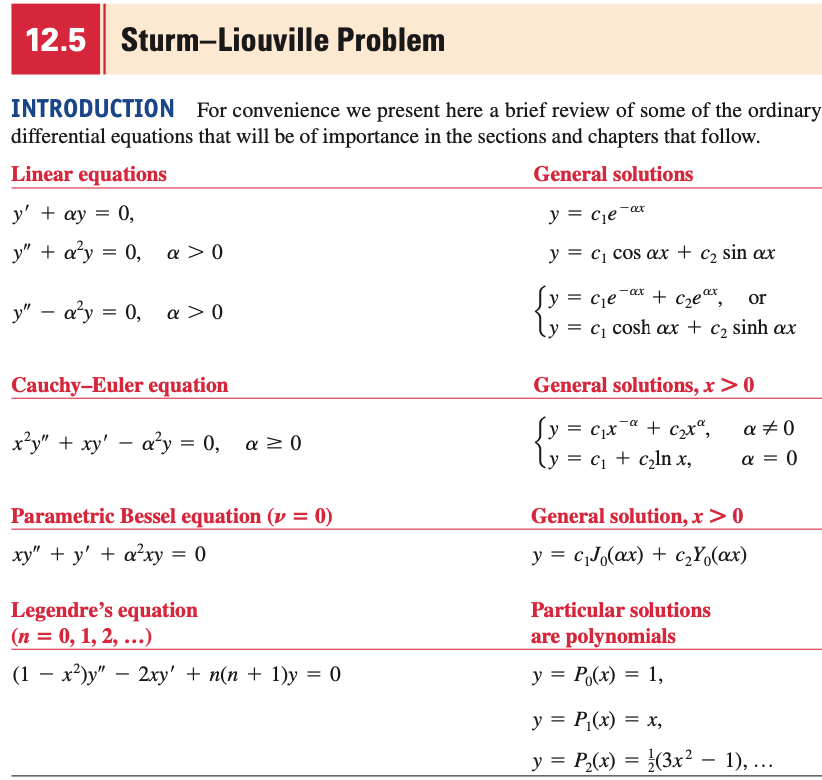
\includegraphics[scale=0.5]{/Users/rudiks/Git/EcuacionesDiferenciales2/Cheatsheet3/Imagenes/Ordinary.png}
\end{center}

\begin{center}
	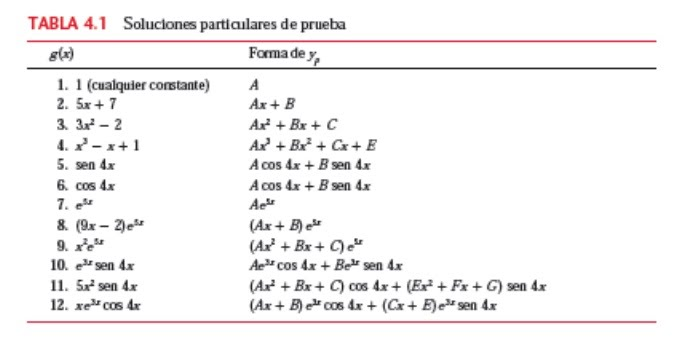
\includegraphics[scale=0.7]{/Users/rudiks/Git/EcuacionesDiferenciales2/Cheatsheet3/Imagenes/Coeficientes.jpg}
\end{center}

\section{Series de Fourier}

\begin{center}
	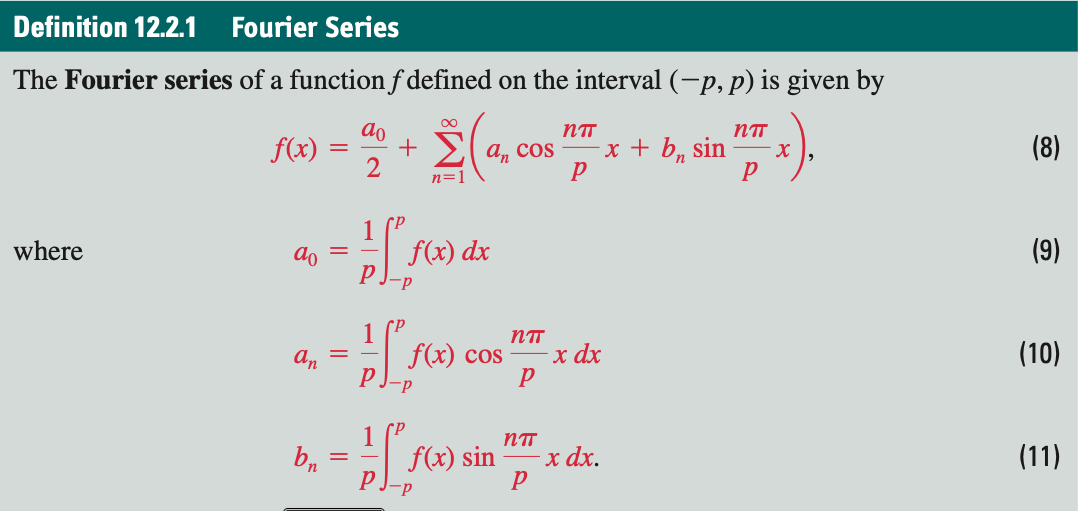
\includegraphics[scale=0.4]{/Users/rudiks/Git/EcuacionesDiferenciales2/Cheatsheet3/Imagenes/Fourier.png}
\end{center}

\begin{center}
	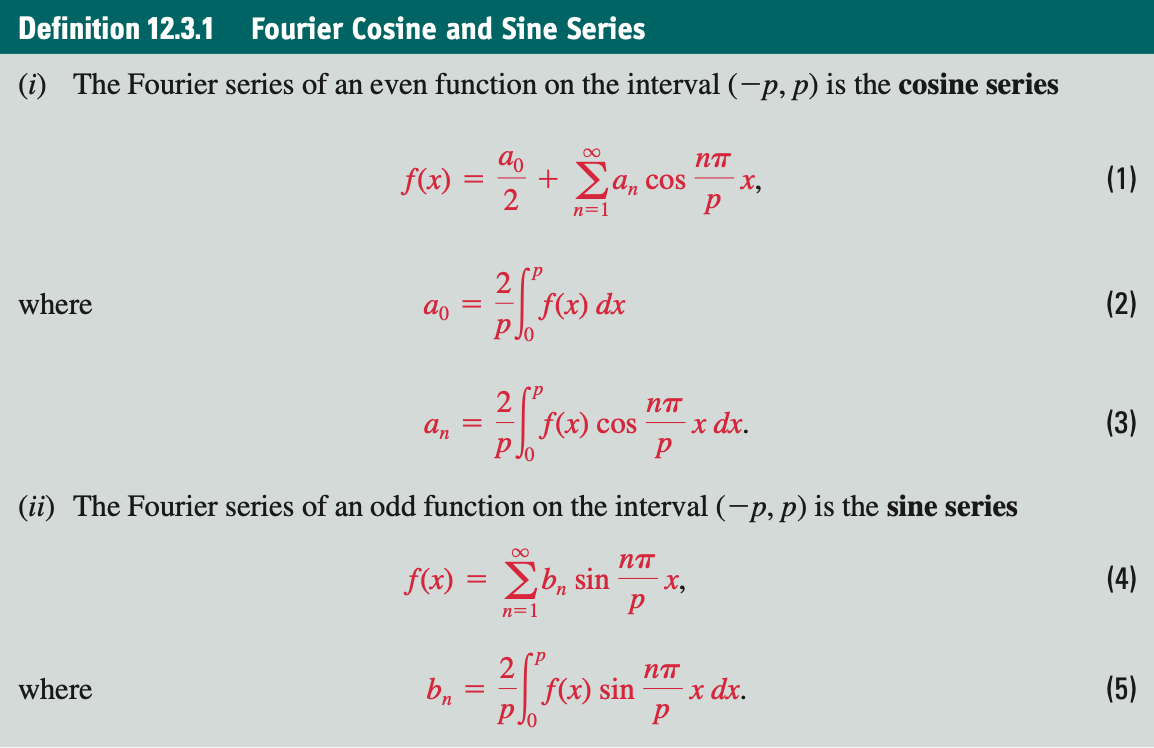
\includegraphics[scale=0.4]{/Users/rudiks/Git/EcuacionesDiferenciales2/Cheatsheet3/Imagenes/Fourier-sin-cos.png}
\end{center}

\newpage 

\section{Integral de Fourier}

\begin{center}
	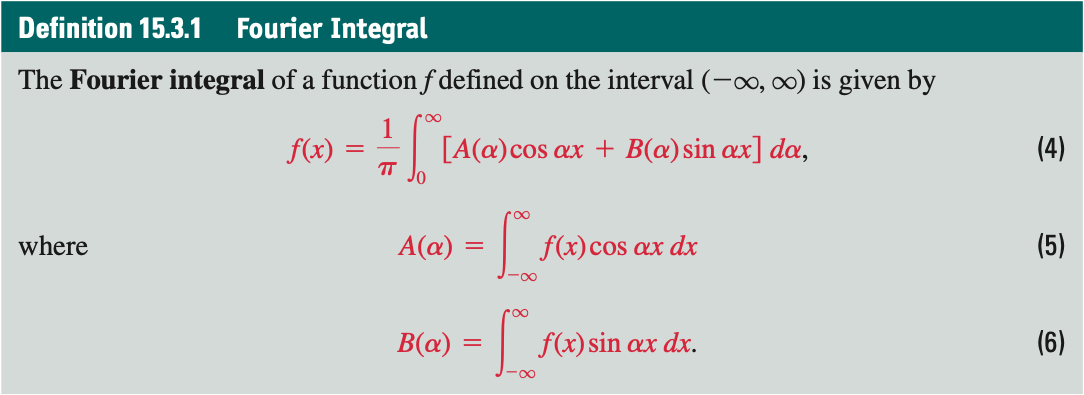
\includegraphics[scale=0.4]{/Users/rudiks/Git/EcuacionesDiferenciales2/Cheatsheet2/Imagenes/Screen Shot 2021-05-05 at 12.16.48.png}
\end{center}
\begin{center}
	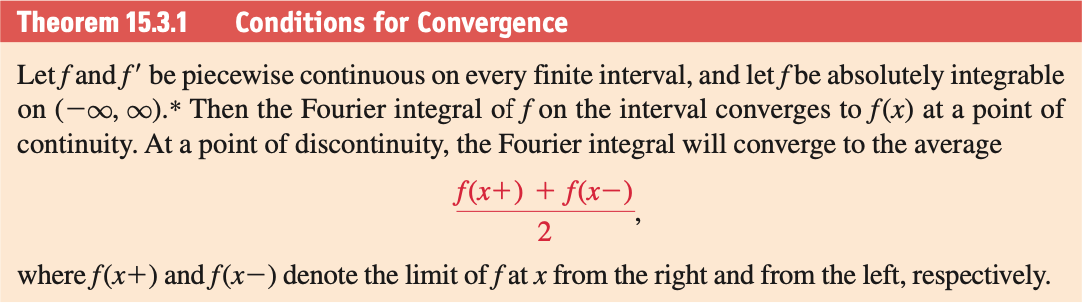
\includegraphics[scale=0.4]{/Users/rudiks/Git/EcuacionesDiferenciales2/Cheatsheet2/Imagenes/Screen Shot 2021-05-05 at 12.16.59.png}
\end{center}
\begin{center}
	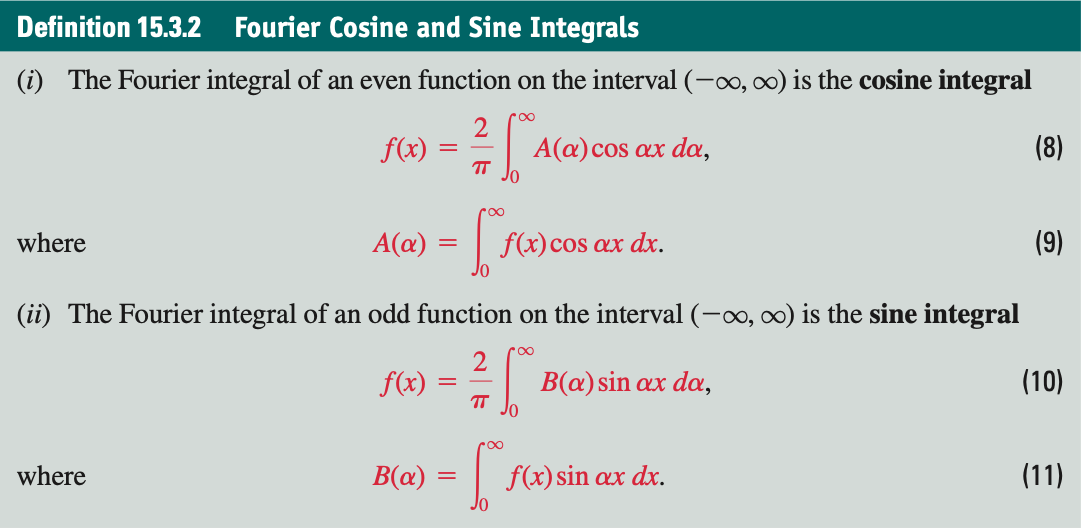
\includegraphics[scale=0.4]{/Users/rudiks/Git/EcuacionesDiferenciales2/Cheatsheet2/Imagenes/Screen Shot 2021-05-05 at 12.17.18.png}
\end{center}

\section{Transformada de Fourier}

\begin{center}
	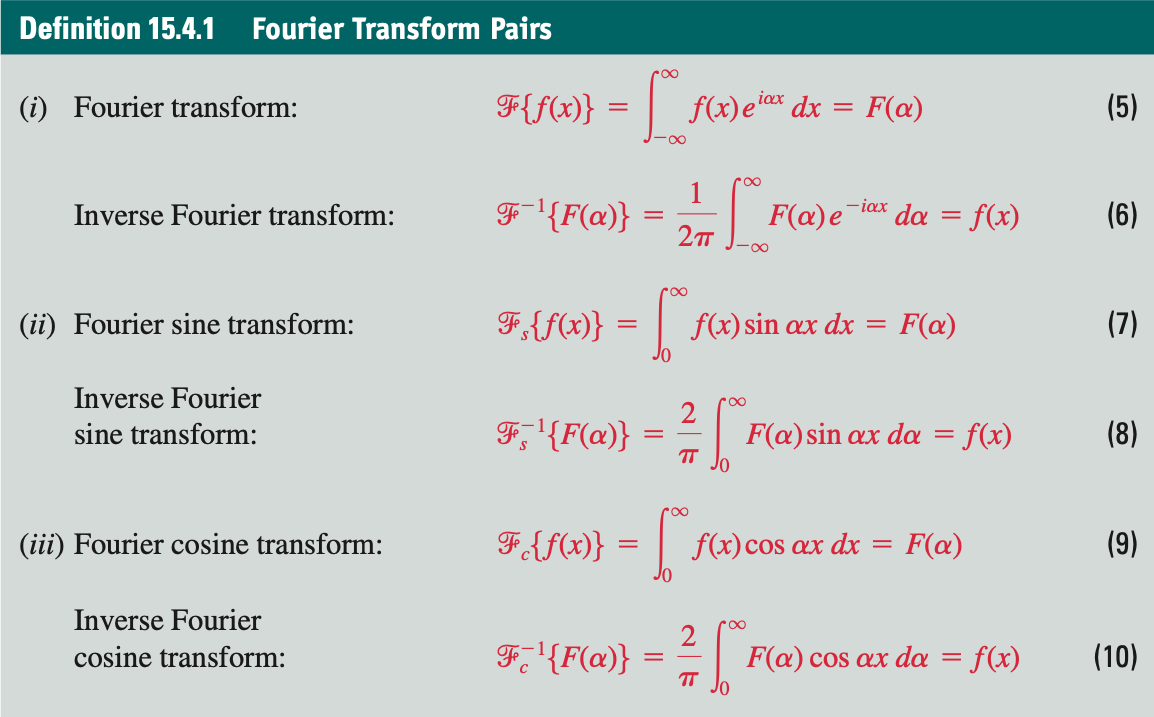
\includegraphics[scale=0.4]{/Users/rudiks/Git/EcuacionesDiferenciales2/Cheatsheet2/Imagenes/Screen Shot 2021-05-07 at 10.35.22.png}
\end{center}

\begin{center}
	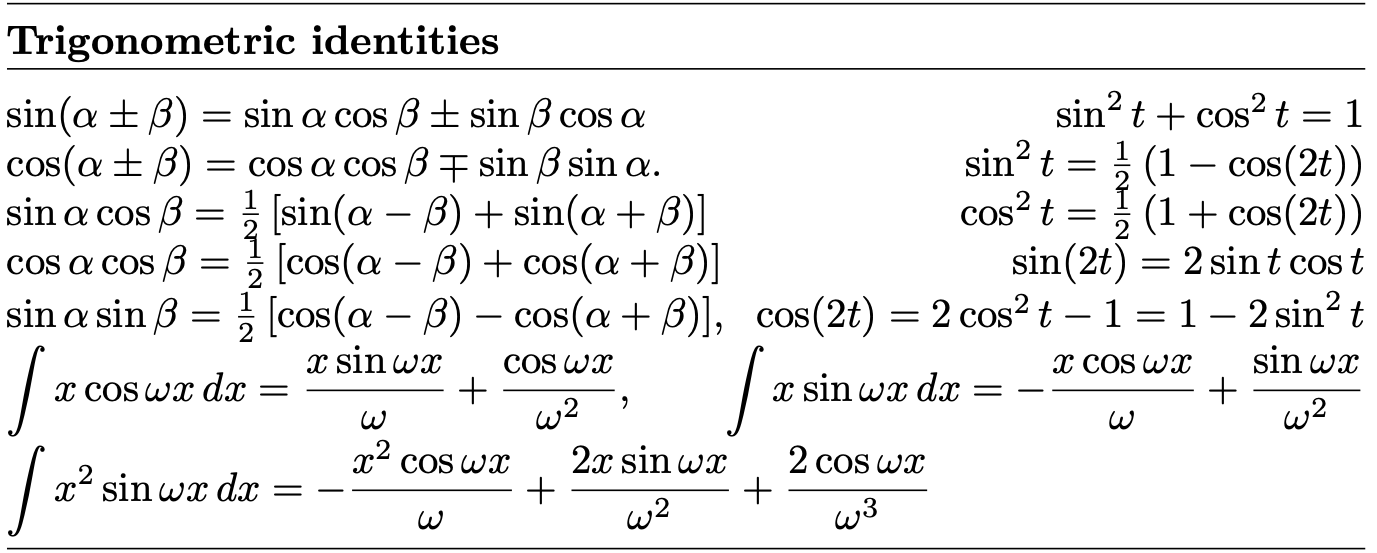
\includegraphics[scale=0.35]{/Users/rudiks/Git/EcuacionesDiferenciales2/Cheatsheet3/Imagenes/Trigonometricas.png}
\end{center}

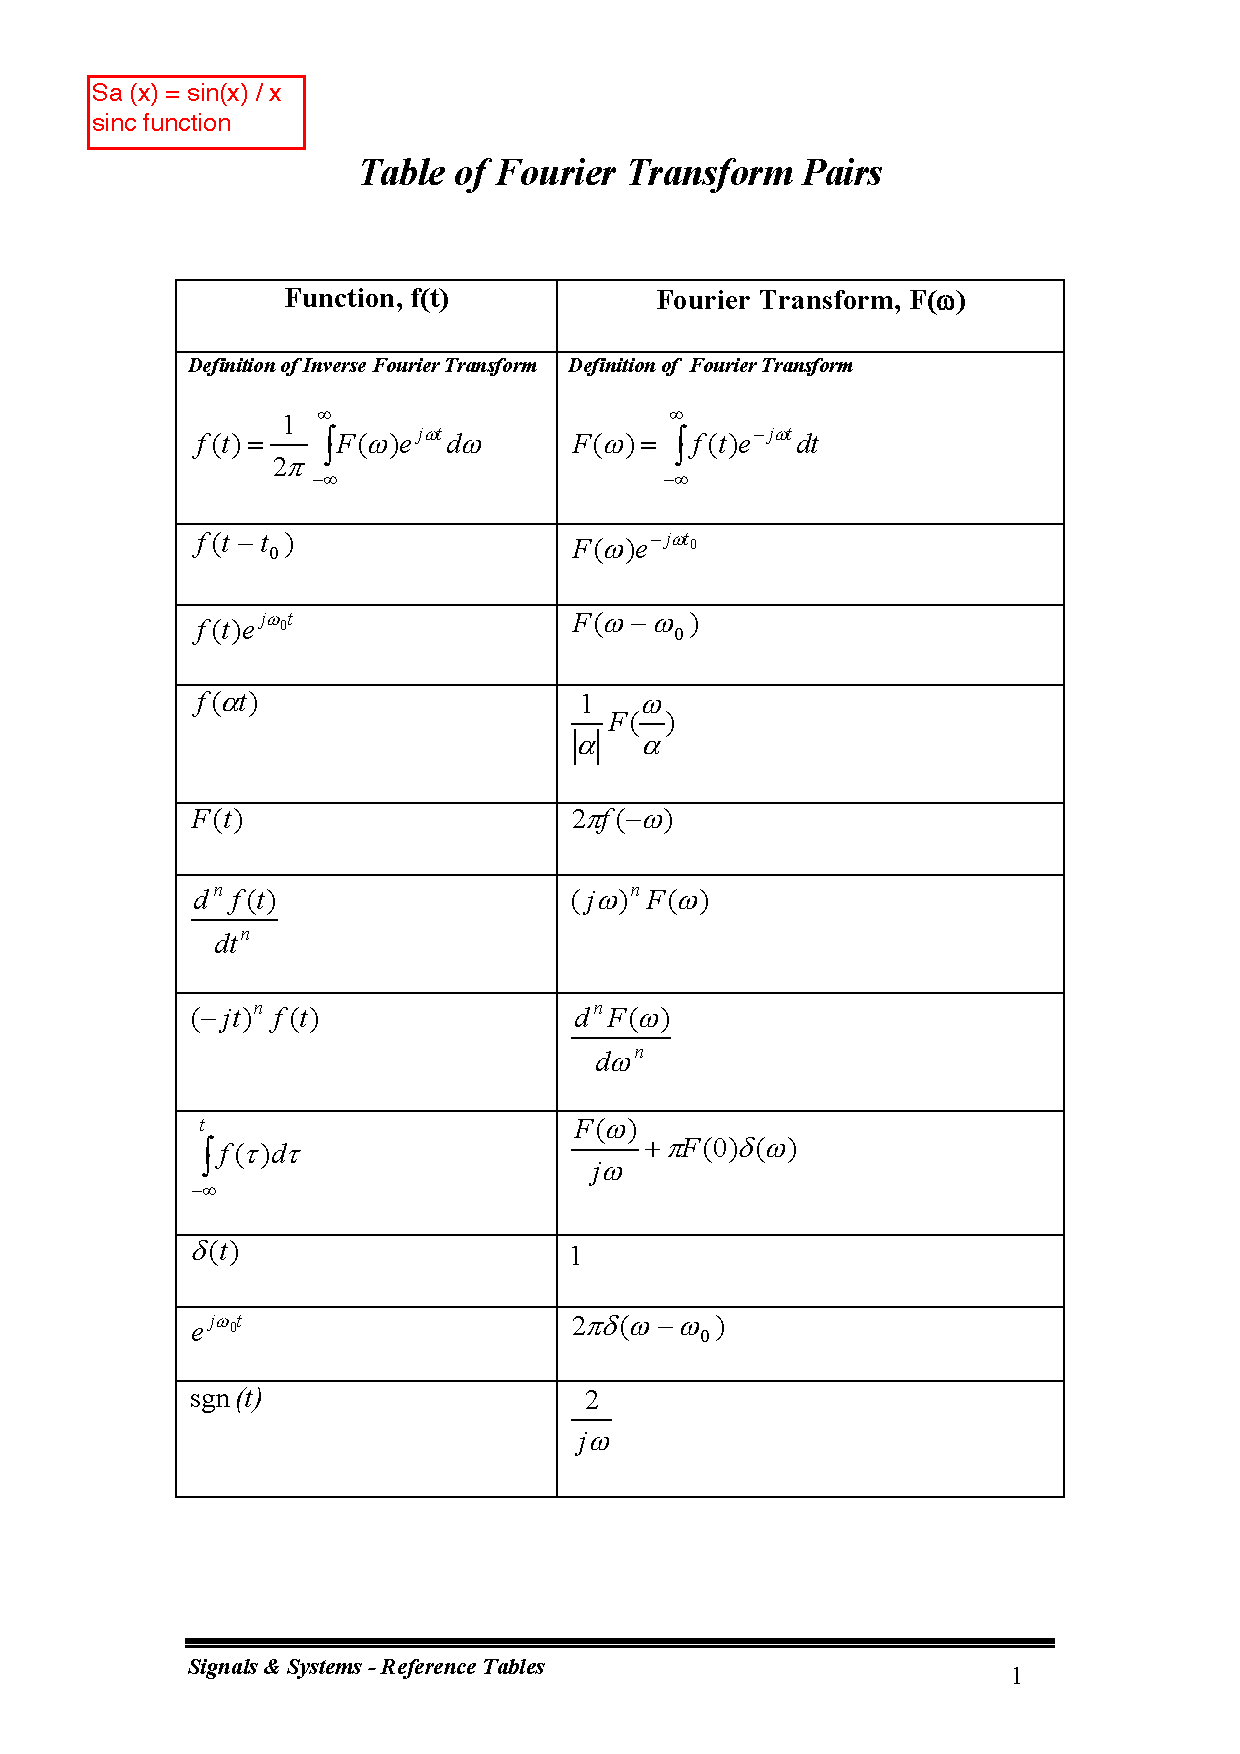
\includepdf[pages=-]{/Users/rudiks/Git/EcuacionesDiferenciales2/Cheatsheet3/Imagenes/FFT table.pdf}

\section{Laplace}
\begin{enumerate}
	\item $\mathcal{L}[u'(x,t)]=s\mathcal{L}[u(x,t)]-u(x,0).$
	\item $\mathcal{L}[u'(x,t)]=s^2\mathcal{L}[u(x,t)]-su(x,0)-u'(x,0).$
	\item$\mathcal{L}\left[\frac{e^{-a\sqrt{s}}}{s}\right]=\operatorname{erfc}\left(\frac{a}{2\sqrt{t}}\right).$
	\item $\mathcal{L}\left[e^{-a\sqrt{s}}\right]=\frac{a}{2\sqrt{\pi t^3}}e^{-\alpha ^2 /4t}, \qquad a>0.$
	\item  $\mathcal{L}\left[\frac{e^{-a\sqrt{s}}}{\sqrt{s}}\right]=\frac{1}{\sqrt{\pi t}}e^{-\alpha ^2 /4t}$
\end{enumerate}

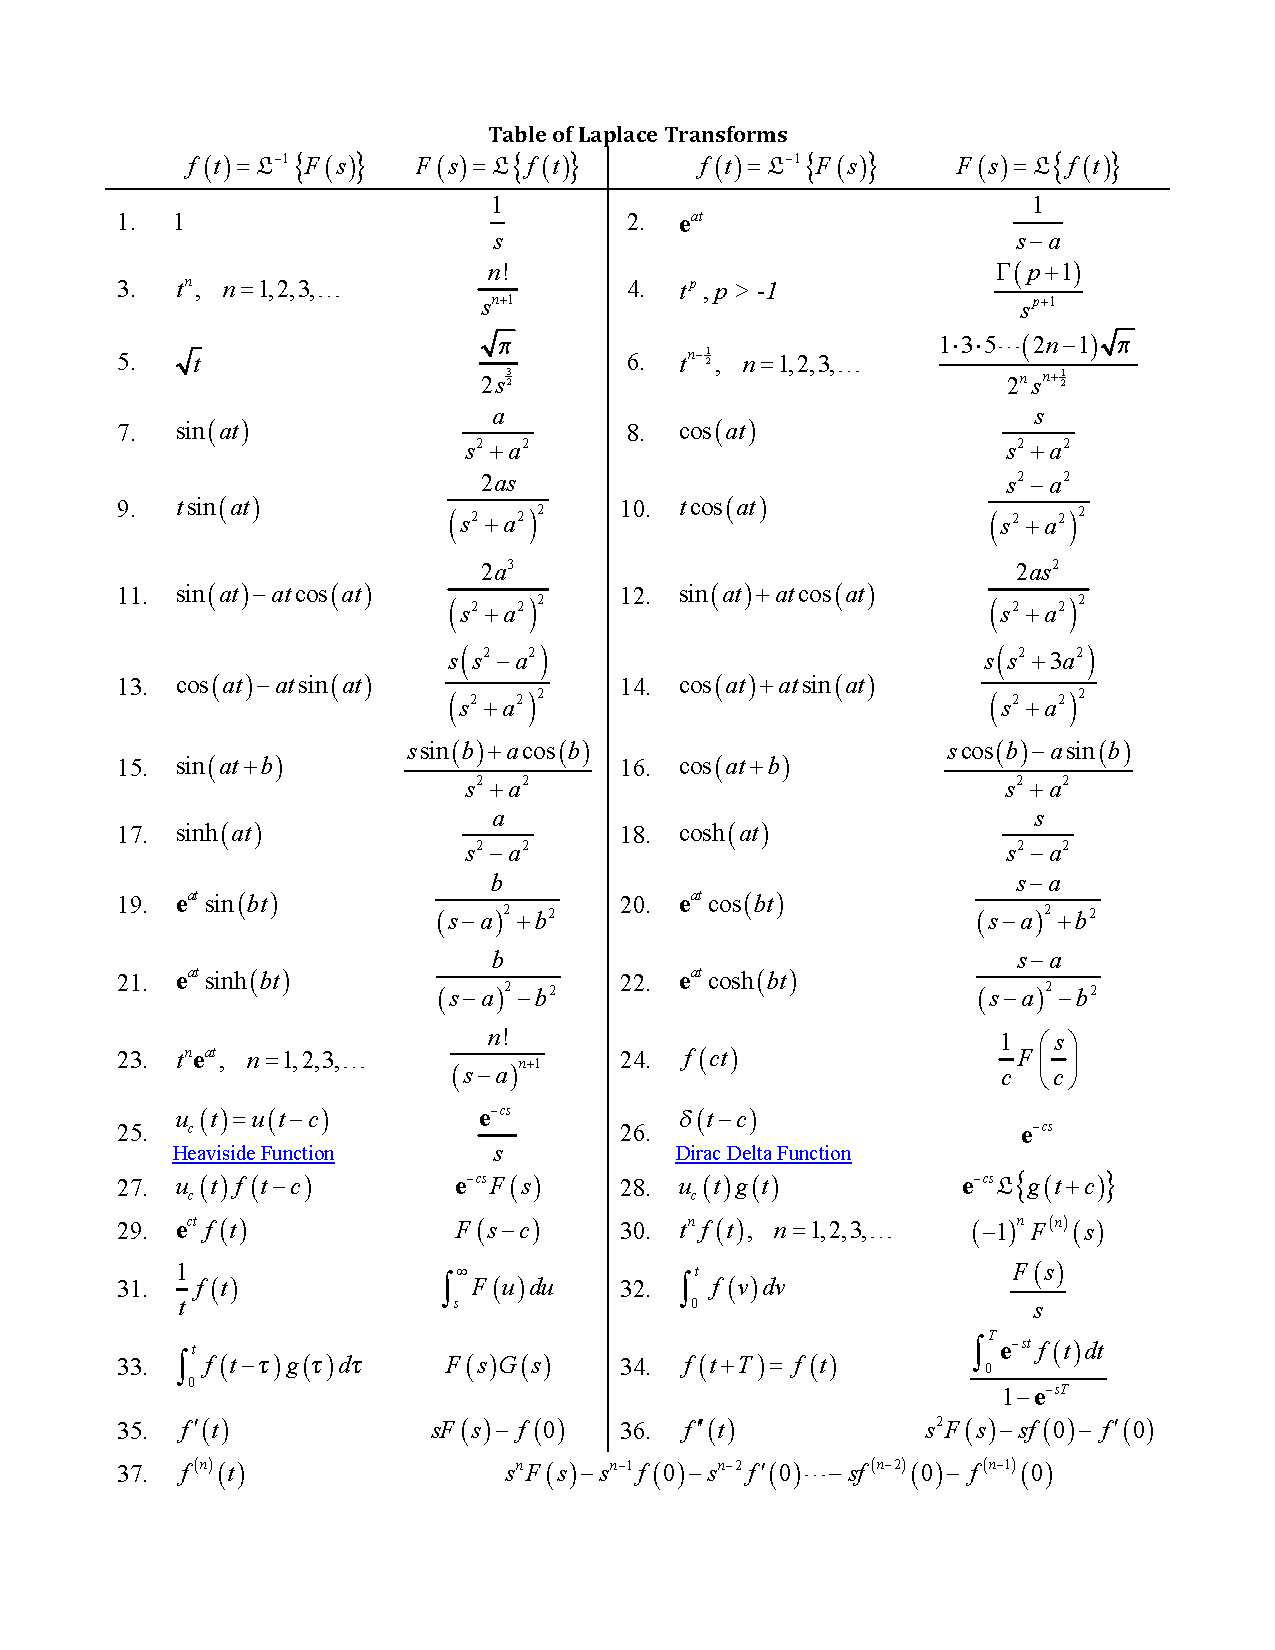
\includepdf[pages=-]{/Users/rudiks/Git/EcuacionesDiferenciales2/Cheatsheet3/Imagenes/Laplace.pdf}
%---------------------------
%\bibliographystyle{apalike}
%\bibliography{sample.bib}

\end{document}